\documentclass{article}
\usepackage{graphicx} % Required for inserting images

\title{Maxwell's Equations}
\author{Sreya A ch22b119}
\begin{document}

\maketitle

\section{Maxwell First Equation}
Maxwell’s first equation is based on the Gauss law of electrostatic, which states that “when a closed surface integral of electric flux density is always equal to charge enclosed over that surface”\\

\begin{align*}
\parindent 0px
\text{Gauss's Law for Electric Field:} \quad & \nabla \cdot \mathbf{E} = \frac{\rho}{\varepsilon_0} \\
\end{align*}

\section{Maxwell Second Equation}
Maxwell second equation is based on Gauss law on magnetostatics.
Gauss law on magnetostatics states that “closed surface integral of magnetic flux density is always equal to total scalar magnetic flux enclosed within that surface of any shape or size lying in any medium.”\\\\
\begin{align*}
\parindent 0px
    \text{Gauss's Law for Magnetic Field:} \quad & \nabla \cdot \mathbf{B} = 0 \\
\end{align*}

\section{Maxwell Third Equation}
Maxwell’s 3rd equation is derived from Faraday’s laws of Electromagnetic Induction. It states that “Whenever there are n-turns of conducting coil in a closed path placed in a time-varying magnetic field, an alternating electromotive force gets induced in each coil.” Lenz’s law gives this. Which states, ” An induced electromotive force always opposes the time-varying magnetic flux.”\\\\
\begin{align*}
\parindent 0px
    \text{Faraday's Law:} \quad & \nabla \times \mathbf{E} = -\frac{\partial \mathbf{B}}{\partial t} \\
\end{align*}

\section{Maxwell Fourth Equation}
It is based on Ampere’s circuit law. To understand Maxwell’s fourth equation, it is crucial to understand Ampere’s circuit law,
Consider a wire of a current-carrying conductor with the current I. Since there is an electric field, there has to be a magnetic field vector around it. Ampere’s circuit law states that “The closed line integral of magnetic field vector is always equal to the total amount of scalar electric field enclosed within the path of any shape”, which means the current flowing along the wire(which is a scalar quantity) is equal to the magnetic field vector (which is a vector quantity)\\\\
\begin{align*}
\parindent 0px
   \text{Ampere's Law with Maxwell's Addition:} \quad & \nabla \times \mathbf{B} = \mu_0 \left(\mathbf{J} + \varepsilon_0 \frac{\partial \mathbf{E}}{\partial t}\right)
\end{align*}\\

Although Maxwell’s most important equations had already appeared throughout his seminal paper entitled “On Physical Lines of Force” , which was written in 1861, it was not until 1864 that Maxwell created a distinct listing of eight equations in his follow up paper known as “A Dynamical Theory of the Electromagnetic Field”. This was in a section headed as ‘General Equations of the Electromagnetic Field’. While Maxwell refers to twenty equations at the end of this section, there are in fact only eight equations as such.\cite{ref=article}\\\\
Maxwell Equation Graph in 3D\\
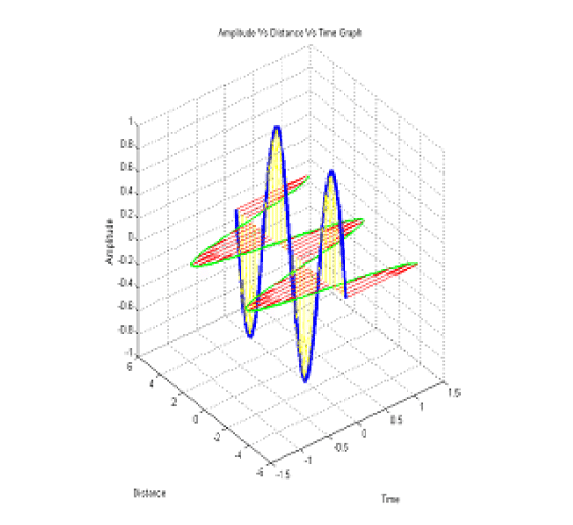
\includegraphics[width=8cm]{Graph-in-3D.png}

\footnote{Reference: Introduction To Electrodynamics David J. Griffiths }

\newpage
\bibliography{maxwell}
\bibliographystyle{plain}
\end{document}
